\section{Kommunikationsenhet}

Kommunikationsenheten ansvarar för att förmedla information mellan de olika enheterna i systemet. 
Kommunikationen mellan PC och roboten kommer att ske via bluetooth. Kommunikation mellan de olika delsystemen på roboten kommer att ske med en så kallad SPI-buss.

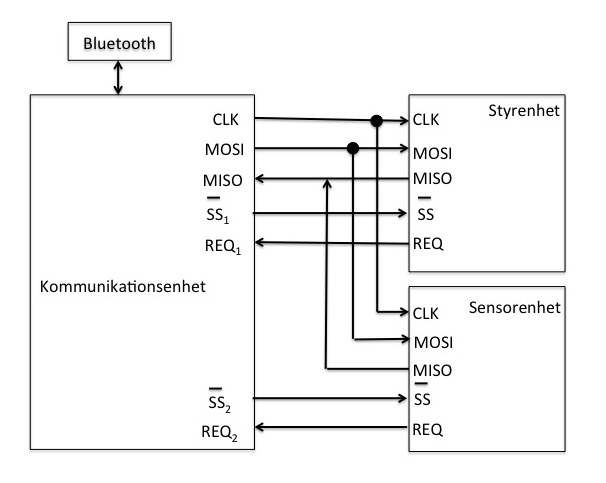
\includegraphics[angle=0,scale=0.5]{bilder/SPI-buss.png}



\subsection{SPI}
SPI bussen är ett kommunikationssystem som använder ett så kallat Master-Slav system. I roboten kommer kommunikationsenheten att vara Master. Systemet kommer att ha två slavar i form av styrenheten och sensorenheten.
Detta betyder att all kommunikation kommer att behöva gå via kommunikationsenheten. SPI bussen arbetar alltid i så kallat full duplex läge vilket betyder att överföringar kan ske i två riktningar samtidigt. Således kan en 2 bits skickas via SPI bussen på 1 klockcykel. 

Robotens kommunikationssystem kommer att fungera så att styr- och sensorenheten har möjlighet att ta initiativ till kommunikation med kommunikationsenheten. Detta är inte standard på SPI-bussen utan löses med två stycken extrasignaler vi kallar för REQ-signaler. Alla sorters kommunikation kommer att styras med hjälp av avbrott, som är ett utmärkt sätt att hantera plötsliga externa kommandon. REQ signalen kommer att generera ett avbrott hos mastern som i sin tur kommer att generera ett avbrott på enheten som skickat REQ signalen. Då mastern initierar kontakten kommer ett avbrott att genereras på den valda enheten. Alla SPI-överföringar avslutas med att en speciell avbrottsflagga kallad (SPIF) sätts.

För att klargöra vart informationen som skickas till Mastern ska sändas kommer det att användas en så kallad header. Detta är en byte med information som specificerar vilken typ av information som skickas och vad som är målet. Som ett exempel kan vi föreställa oss att roboten är inne i en labyrint. 

Nedan följer klargöranden om hur projektgruppen ämnar använda de olika portarna i SPI-bussen. 


\subsubsection{CLK}

CLK porten är en port som förmedlar en klocka med en viss frekvens från Mastern till de två slavarna. Denna signal bestämmer hur snabbt överföringen ska ske. Denna klocka behöver inte nödvändigtvis vara samma som masterenhetens arbetsklocka. 

\subsubsection{MOSI}
MOSI porten är den port som används när kommunikationsenheten ska förmedla information till styrenheten och sensorenheten. Den kommer att användas som input för slavarna och output för mastern. Den information som kommer att skickas beror på i vilket läge roboten arbetar i. I manuellt läge kommer det genom MOSI portarna förmedlas styrinformation till styrenheten som kommunikationsenheten i sin tur får från en PC via bluetooth. I autonomt läge kommer här till exempel att skickas data som sensorenheten använder vid regleringsalgoritmen. Annan information som kommer att skickas via MOSI är specialbeslut, till exempel om roboten måste svänga 90\degree i en labyrint.

\subsubsection{MISO}
MISO porten kommer att konfigureras att fungera som den port som används då kommunikationsenheten hämtar information från styr- och sensorenheten. Den kommer alltså att vara en input för mastern och output för båda slavarna. Exempel på information som ska skickas med MISO är data som skickas från sensorenheten för vidare transport till styrenheten. Ett annat exempel är i autonomt läge när roboten befinner sig i en labyrint. Då kommer här att skickas information om vilka beslut sensorenheten. Dessa beslut skickas sedan vidare till en PC via bluetooth.
Då all kommunikation med SPI är tvåsidig kommer även MOSI porten att användas varje gång MISO porten används, och vice versa. Finns det inget intresse av dubbelsidig kommunikation finns möjligheterna att ignorera den skickade informationen.

\subsubsection{SS}
SS portarna skickar eller tar emot en variant på en chip-select . Den SS signal som är låg väljer vilken av slavarna som mastern ska kommunicera med. Endast en av de två SS portarna kan vara låg samtidigt. Dessa portar kommer att vara output på kommunikationsenheten och input på de styr- och sensorenheten.
När SS signalen till en av slavarna är låg betyder det alltså att slavens SPI är aktiverad. Ett avbrott kommer att göras på den valda slaven och när olika konfigurationer utförts kommer information att börja skickas från kommunikationsenheten till den enhet som har en låg SS signal. Kommunikation kommer som sagt samtidigt att ske åt andra riktningen också. Under tiden kommer den enhet som får en hög SS signal att vara omöjlig att kommunicera med.
När sändningen är klar sätts SPI avbrottsflaggan (SPIF) i både mastern(kommunikationsenheten) och slaven(någon av styr- eller sensorenheten). Detta avbrott berättar att överföringen är färdig och SS signalen återigen kan sättas hög av kommunikationsenheten.







